\begin{frame}
  \frametitle{\textbf{Jet suppression}}
  \begin{columns}
    \column{0.5\textwidth}
    \begin{itemize}
    \item Leading hadron measurements do not fully connect to the initial fragmenting parton
    \item Suppression of fully reconstructed jets is a better probe
      \begin{itemize}
      \item Weak $p_{\text{T}}$ dependence
      \item Scales with centrality
      \end{itemize}
    \end{itemize}
    \begin{align*}
      R_{\text{AA}}^{\text{jet}} (p_{\text{T}}) = \cfrac{dN^{\text{AA}}_{\text{jet}} / dp_{\text{T}}}{\left< N_{\text{coll}} \right> dN^{\text{pp}}_{\text{jet}} / dp_{\text{T}}}
    \end{align*}
    \column{0.5\textwidth}
    \begin{tikzpicture}
      \node{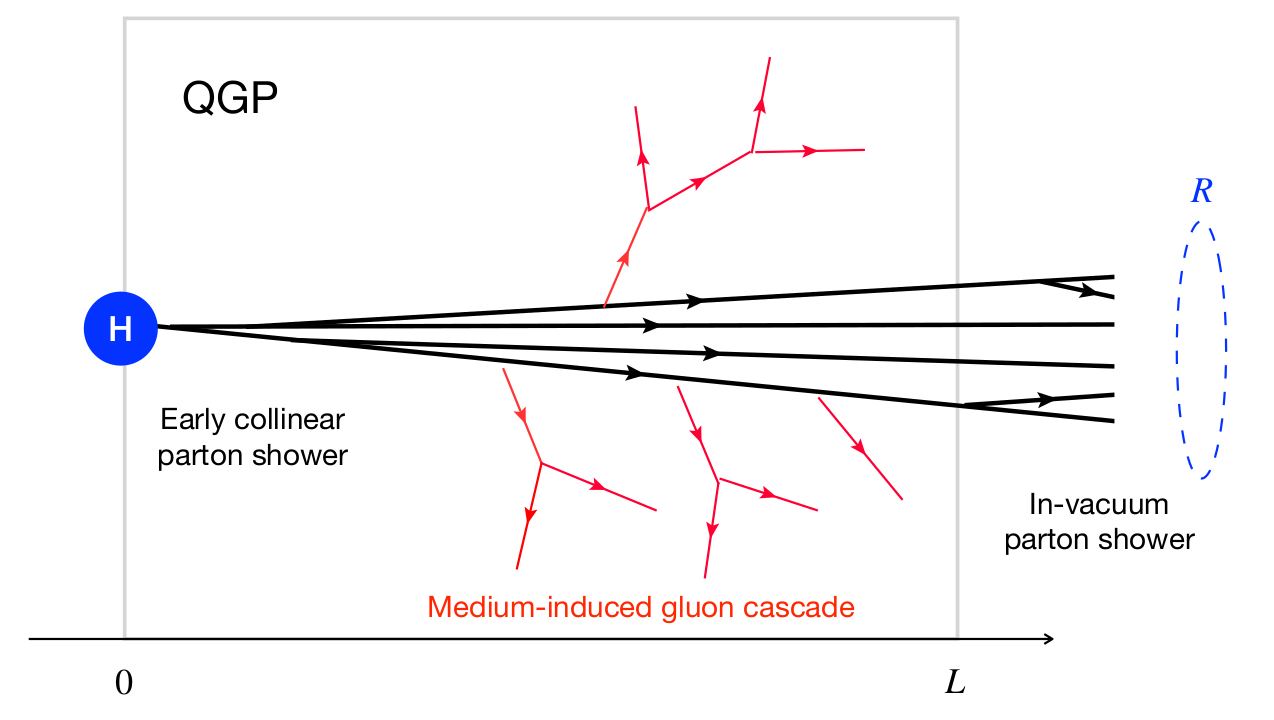
\includegraphics[width=\textwidth]{jet-suppression-cartoon.png}};
    \end{tikzpicture}
  \end{columns}
  \begin{columns}
    \column{0.5\textwidth}
    \begin{tikzpicture}
      \node{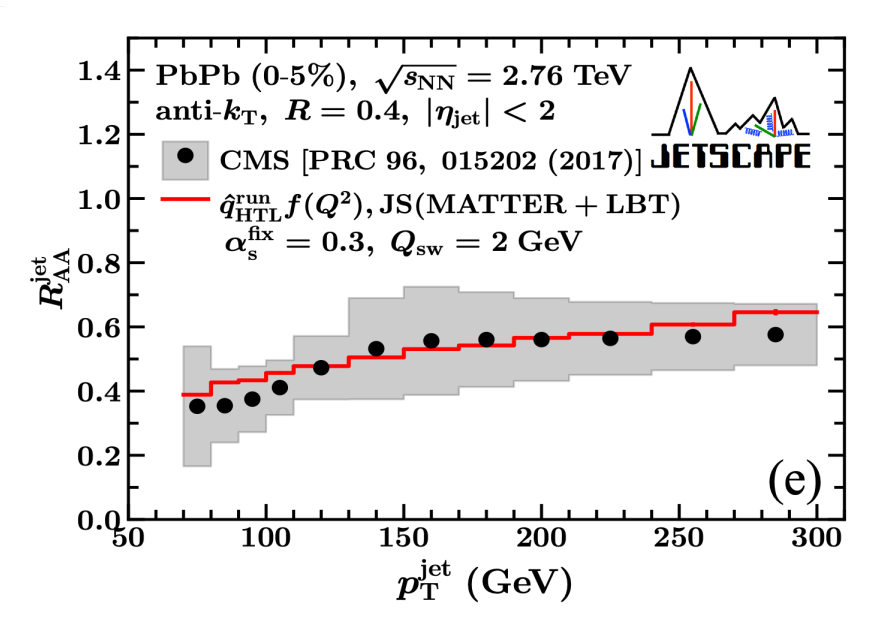
\includegraphics[width=\textwidth]{jet-RAA.png}};
    \end{tikzpicture}
    \column{0.5\textwidth}
    \begin{tikzpicture}
      \node{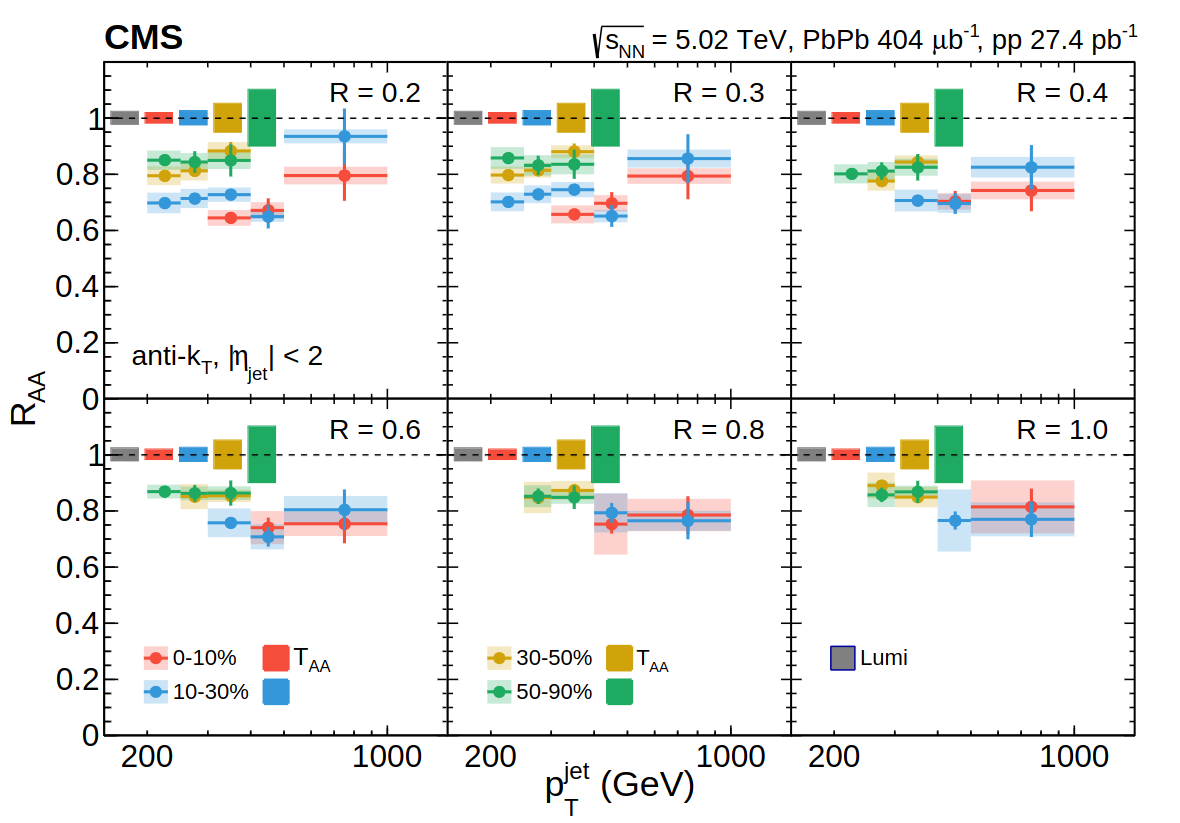
\includegraphics[width=\textwidth]{jet-radii-RAA.png}};
    \end{tikzpicture}
  \end{columns}
\end{frame}
